\documentclass[a4paper]{article}
\usepackage{a4wide,amssymb,epsfig,latexsym,multicol,array,hhline,fancyhdr}
\usepackage{vntex}
\usepackage{amsmath}
\usepackage{lastpage}
\usepackage[lined,boxed,commentsnumbered]{algorithm2e}
\usepackage{enumerate}
\usepackage{color}
\usepackage{graphicx}							% Standard graphics package
\usepackage{array}
\usepackage{tabularx, caption}
\usepackage{multirow}
\usepackage{multicol}
\usepackage{rotating}
\usepackage{graphics}
\usepackage{geometry}
\usepackage{setspace}
\usepackage{epsfig}
\usepackage{tikz}
\usetikzlibrary{arrows,snakes,backgrounds}
\usepackage{hyperref}
\hypersetup{urlcolor=blue,linkcolor=black,citecolor=black,colorlinks=true} 
%\usepackage{pstcol} 								% PSTricks with the standard color package

\newtheorem{theorem}{{\bf Theorem}}
\newtheorem{property}{{\bf Property}}
\newtheorem{proposition}{{\bf Proposition}}
\newtheorem{corollary}[proposition]{{\bf Corollary}}
\newtheorem{lemma}[proposition]{{\bf Lemma}}

\AtBeginDocument{\renewcommand*\contentsname{Mục lục}}
\AtBeginDocument{\renewcommand*\refname{References}}
%\usepackage{fancyhdr}
\setlength{\headheight}{40pt}
\pagestyle{fancy}
\fancyhead{} % clear all header fields
\fancyhead[L]{
	\begin{tabular}{rl}
		\begin{picture}(25,15)(0,0)
			\put(0,-8){
\includegraphics[width=8mm, height=8mm]{images/hcmut.png}}
			%\put(0,-8){\epsfig{width=10mm,figure=hcmut.eps}}
		\end{picture}&
		%
\includegraphics[width=8mm, height=8mm]{hcmut.png} & %
		\begin{tabular}{l}
			\textbf{\bf \ttfamily Đại học Bách Khoa TP.HCM}\\
			\textbf{\bf \ttfamily Khoa Khoa học và Kĩ thuật Máy tính}
		\end{tabular} 	
	\end{tabular}
}
\fancyhead[R]{
	\begin{tabular}{l}
		\tiny \bf \\
		\tiny \bf 
\end{tabular}  }
\fancyfoot{} % clear all footer fields
\fancyfoot[L]{\scriptsize \ttfamily Bài tập lớn môn Mạng Máy Tính (CO3093) - Năm học 2023 - 2024}
\fancyfoot[R]{\scriptsize \ttfamily Trang {\thepage}/\pageref{LastPage}}
\renewcommand{\headrulewidth}{0.3pt}
\renewcommand{\footrulewidth}{0.3pt}


%%%
\setcounter{secnumdepth}{4}
\setcounter{tocdepth}{3}
\makeatletter
\newcounter {subsubsubsection}[subsubsection]
\renewcommand\thesubsubsubsection{\thesubsubsection .\@alph\c@subsubsubsection}
\newcommand\subsubsubsection{\@startsection{subsubsubsection}{4}{\z@}%
	{-3.25ex\@plus -1ex \@minus -.2ex}%
	{1.5ex \@plus .2ex}%
	{\normalfont\normalsize\bfseries}}
\newcommand*\l@subsubsubsection{\@dottedtocline{3}{10.0em}{4.1em}}
\newcommand*{\subsubsubsectionmark}[1]{}
\makeatother


\begin{document}
	
	\begin{titlepage}
		\begin{center}
			ĐẠI HỌC QUỐC GIA TP.HCM \\
			ĐẠI HỌC BÁCH KHOA TP.HCM \\
			KHOA KHOA HỌC VÀ KĨ THUẬT MÁY TÍNH
		\end{center}
		
		\vspace{1cm}
		
		\begin{figure}[h!]
			\begin{center}
				
\includegraphics[width=3cm]{images/hcmut.png}
			\end{center}
		\end{figure}
		
		\vspace{1cm}
		
		
		\begin{center}
			\begin{tabular}{c}
				\multicolumn{1}{l}{\textbf{{\Large MẠNG MÁY TÍNH (CO3093)}}}\\
				~~\\
				\hline
				\\
				\multicolumn{1}{l}{\textbf{{\Large Assignment 1}}}\\
				\\
				\textbf{{\Huge Develop a Network Application}}\\
				\\
				\hline
			\end{tabular}
		\end{center}
		
		\vspace{3cm}
		
		\begin{table}[h]
			\begin{tabular}{rrl}
				\hspace{5 cm} & Giảng viên hỗ trợ: & Nguyễn Phương Duy\\
				& Students: & Fullname of Student 1 - Student 1 ID numbers. \\
				& & Fullname of Student 2 - Student 2 ID numbers. \\
			\end{tabular}
		\end{table}
		
		\begin{center}
			{\footnotesize Thành phố Hồ Chí Minh, Tháng 12 năm 2020}
		\end{center}
	\end{titlepage}
	
	
	%\thispagestyle{empty}
	
	\newpage
	\tableofcontents
	\newpage
	
	
	%%%%%%%%%%%%%%%%%%%%%%%%%%%%%%%%%
	\section{Member list \& Workload}
	
	\begin{center}
		\begin{tabular}{|c|c|c|l|c|}
			\hline
			\textbf{No.} & \textbf{Fullname} & \textbf{Student ID} & \textbf{Problems} & \textbf{Percentage of work}\\
			\hline 
			%%%%%Student 1%%%%%%%%%%
			\multirow{3}{*}{1} & \multirow{3}{*}{Nguyễn Văn A} & \multirow{3}{*}{19181716} & - Relation \& Counting: 1, 2, 3& \multirow{3}{*}{30\%}\\
			& &  & Bonus: 1, 2, 3. &\\
			& &  & - Probability: 1, 2, 3. &\\
			\hline 
			%%%%%Student 2%%%%%%%%%%%
			\multirow{3}{*}{2} & \multirow{3}{*}{Nguyễn Văn B} & \multirow{3}{*}{19181717} & - Relation \& Counting: 4, 5, 6& \multirow{3}{*}{20\%}\\
			& &  & Bonus: 4, 5, 6. &\\
			& &  & - Graph: 1, 2, 3, Bonus: 1, 2, 3. &\\
			\hline
			%%%%%Student 3%%%%%%%%%%%
		\end{tabular}
	\end{center}
	
	%%%%%%%%%%%%%%%%%%%%%%%%%%%%%%%%%
	\section{Application specifications and requirements}
	\subsection{Project objectives}
	$\indent$Mục đích của bài tập lớn môn Mạng Máy tính học kì 1 năm học 2023-2024 là xây dựng một chương trình chia sẻ file đơn giản, với giao thức chương trình do mỗi nhóm quyết định, dựa trên các giao thức TCP/IP đã học.
	
	\subsection{Project specifications and description}
	$\indent$ Mô tả chương trình trong đề bài bài tập lớn 1:
	\begin{itemize}
		\item Một máy chủ (server) trung tâm đóng vai trò theo dõi, quản lí các client đã kết nối và các file mà chúng giữ.
		\item Một client sẽ thông báo cho server biết có những file gì trong thư mục tại chổ (local repository) nhưng sẽ không truyền những file đó cho server.
		\item Khi một client cần một file không nằm trong thư mục của nó, môt yêu cầu sẽ được gửi đến server. Server có nhiệm vụ xác định những clients khác có chứa file được yêu cầu và gửi thông tin kết nối của chúng đến client yêu cầu. Client đó sẽ lựa chọn nguồn lấy phù hợp và tiến hành nhận file trực tiếp từ đó mà không qua can thiệp của server. (Loại mạng kết nối Peer-to-peer)
		\item Nhiều client có thể tải nhiều file khác nhau từ cùng một client gốc tại bất kì thời điểm nào
		\item Client có giao diện câu lệnh (Command line interface - CLI) đơn giản nhận hai câu lệnh:
		\begin{itemize}
			\item \textbf{publish \textit{lname fname}}: một file trong file system của client đã được thêm vào local repository của client đó và thông tin này được truyền đến cho server.
			\item \textbf{fetch \textit{fname}}: lấy một bản copy từ file mục tiêu và thêm nó vào local repository.
		\end{itemize}
		\item Server cũng sẽ có CLI nhận hai câu lệnh:
		\begin{itemize}
			\item \textbf{discover \textit{hostname}}: cho ra danh sách những file trong local repository của \textit{hostname}.
			\item \textbf{ping \textit{hostname}}: kiểm tra trực tiếp \textit{hostname}, tương tự như câu lệnh SNMP ping.
		\end{itemize}
	\end{itemize}
	$\indent$Bên cạnh đó, dựa trên ý kiến của các thành viên, nhóm có thêm các yêu cầu dựa trên các chức năng thêm và cách xử lí khi gặp các trường hợp đăc biệt:
	\begin{itemize}
		\item Với các câu lệnh bên phía client:
		\begin{itemize}
			\item Câu lệnh \textbf{publish \textit{lname fname}} sẽ tiến hành thêm file từ trong máy của client vào local repo và thông báo tới server .Nếu publish một file không tồn tại sẽ báo lỗi "File not exist!". Nếu file publish đã nằm trong local repo sẵn rồi báo "File already in local repo!".
			\item Cách xử lí của câu lệnh \textbf{fetch \textit{fname}} của client trong các trường hợp
			\begin{enumerate}
				\item Nếu file đó không nằm trong hệ thống server quản lí thì báo lỗi "File not recognized!"
				\item Nếu file đó đã nằm trong repo của client thì thông báo đã file đã tồn tại trong local repository
				\item Nếu file đó không nằm trong repo thì thực hiện theo như đề bài yêu cầu
				\item Nếu client chứa file đó không kết nối được thì báo lỗi kết nối 
			\end{enumerate}
			Bên cạnh đó, việc fetch một file vào local repository cũng sẽ đồng thời thông báo với server, tức là file tên \textit{fname} có mặt trên ít nhất hai client.
			\item Thêm câu lệnh \textbf{delete \textit{filename}}: Xóa một file từ local repo ra khỏi hệ thống i.e server sẽ không còn lưu thông tin về file này trên client nữa.
			Báo lỗi "Cannot delete! File not in local repo!" nếu file đó không nằm trong local repo của client yêu cầu. Tức là một client chỉ có thể xóa một file trong local repo của bản thân.
		\end{itemize}
		\item Với câu lệnh bên phía server:
		\begin{itemize}
			\item Lưu ý của câu lệnh \textbf{discover \textit{hostname}}: Nếu một \textit{hostname} chưa từng kết nối với server từ trước thì báo lỗi "Host not recognize!". Nếu \textit{hostname} đã kết nối nhưng chưa publish bất kì file thì báo "\textit{hostname} has not published any files!".
			\item \textbf{ping \textit{hostname}}: Tương tự như câu lệnh ping trong command prompt, gửi vài packet/message nhỏ đến \textit{hostname} rồi chờ phản hồi.
		\end{itemize}
		\item Client sẽ biết trước thông tin kết nối của server.
		\item Client cần có cơ chế tạo, quản lí nhiều cổng kết nối sử dụng đa luồng để nhiều client có thể kết nối với một client.
		\item Các client không cần liên tục kết nối với server để thực hiện việc truyền file, miễn là vẫn nằm trong cùng một network.
		\item Server lưu thông tin về các client đã kết nối cũng như các file họ đã publish trong hệ dữ liệu của chính nó (tức là nếu tắt server đi thì dữ liệu này cũng sẽ biến mất).
		\item Server cũng cần có cơ chế tạo, quản lí nhiều cổng kết nối cùng một lúc.
		\item Có thể có nhiều bản copy của một file trên nhiều client khác nhau. 
		\item Hệ thống không nhận diện các file trùng lặp trong local repo của client. Tức là kể cả khi client có nhiều file trùng lặp thì hệ thống chỉ ghi nhận chỉ một file trong local repo. (\textbf{publish \textit{lname fname}} không cho phép file trùng lặp được publish lên server)
	\end{itemize}
	
	%%%%%%%%%%%%%%%%%%%%%%%%%%%%%%%%%
	\section{System modeling and architecture design}
	\subsection{General use-case diagram}
	$\indent$Hệ thống có 2 actor, bao gồm server và client. Bên cạnh đó, hệ thống cũng có hai module xử lí hai dịch vụ khác nhau của chương trình: quản lí file và client (clients and files management), truyền file (file transfer). Với mỗi module đó là các use-case ứng với mỗi câu lệnh và chức năng của từng actor.
	\begin{figure}[h]
		\begin{center}
			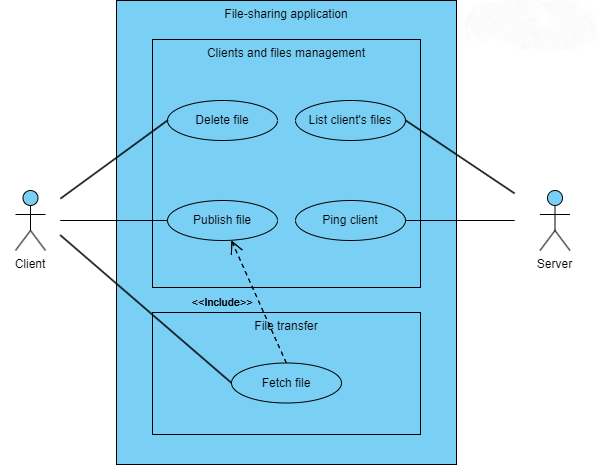
\includegraphics[width=\textwidth]{images/Gen_usecase_diagram.png}
			\hspace{\textwidth}
			\caption{Lược đồ use-case tổng quát}
			\label{usecase_diagram}
		\end{center}
	\end{figure}
	
	\subsection{Class diagram}
	...
	
	\subsection{Activity diagram main functions}
	$\indent$Ứng với mỗi câu lệnh (use-case) chính của từng actor, ta có được các lược đồ hoạt động (activity diagram) dưới đây. Ở đây lưu ý, khi lược đồ đi đến final node thì cũng đồng thời đóng mọi kết nối socket đã thiết lập trước đó, nhằm tránh việc tạo quá nhiều kết nối không cần thiết.
	\subsubsection{publish \textit{lname fname}}
	$\indent$Client sẽ đầu tiên gửi yêu cầu kết nối với server, server sẽ lắng nghe yêu cầu từ một socket đang chạy của mình, thiết lập kết nối giữa client và server. Sau đó, client thực hiện việc publish file lên dữ liệu của server. Kiểm tra tại client file đó có tồn tại không. Nếu có thì tiếp tục use-case, không thì báo lỗi và kết thúc. Sau đó, server sẽ kiểm tra xem client này đã publish file này vào local repo trước đó chưa. Nếu có rồi thì báo lỗi và kết thúc, nếu không thì tiếp tục use-case. Server sẽ thêm file đó vào dữ liệu của mình và client thì thêm file đó vào local repo trên máy. Cuối cùng là đóng kết nối và kết thúc use-case.
	\begin{figure}[!h]
		\begin{center}
			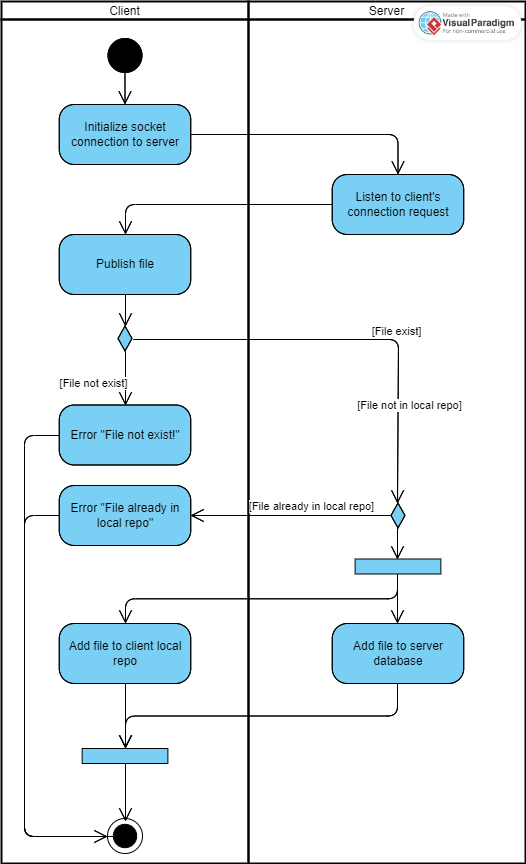
\includegraphics[width=0.6\textwidth]{images/publish_activity_diagram.png}
			\hspace{\textwidth}
			\caption{Lược đồ hoạt động của câu lệnh \textbf{publish \textit{lname fname}}}
			\label{publish_diagram}
		\end{center}
	\end{figure}
	\subsubsection{fetch \textit{fname}}
	$\indent$Thiết lập kết nối tương tự như \textbf{publish}. Tuy nhiên, trong lúc implement thực tế chương trình, nhóm có sửa đổi thứ tự hoạt động khác lược đồ một chút để thuận tiện cho việc code. Trong đó, sau khi client gửi yêu cầu fetch file, server sẽ kiểm tra file đó đã có trong local repo chưa. Nếu có rồi thì báo lỗi và kết thúc, nếu không thì tiếp tục use-case. Sau đó, server tiến hành tìm client có file được yêu cầu. Nếu không tìm được i.e file không nằm trong dữ liệu server thì báo lỗi và kết thúc, còn nếu tìm được thì gửi thông tin kết nối của target client cho client yêu cầu. Sau đó client yêu cầu thiết lập kết nối với target client và tiến hành truyền file. Cuối cùng, đóng mọi socket đã thiêt lập (cả với server và target client).
	\begin{figure}[!h]
		\begin{center}
			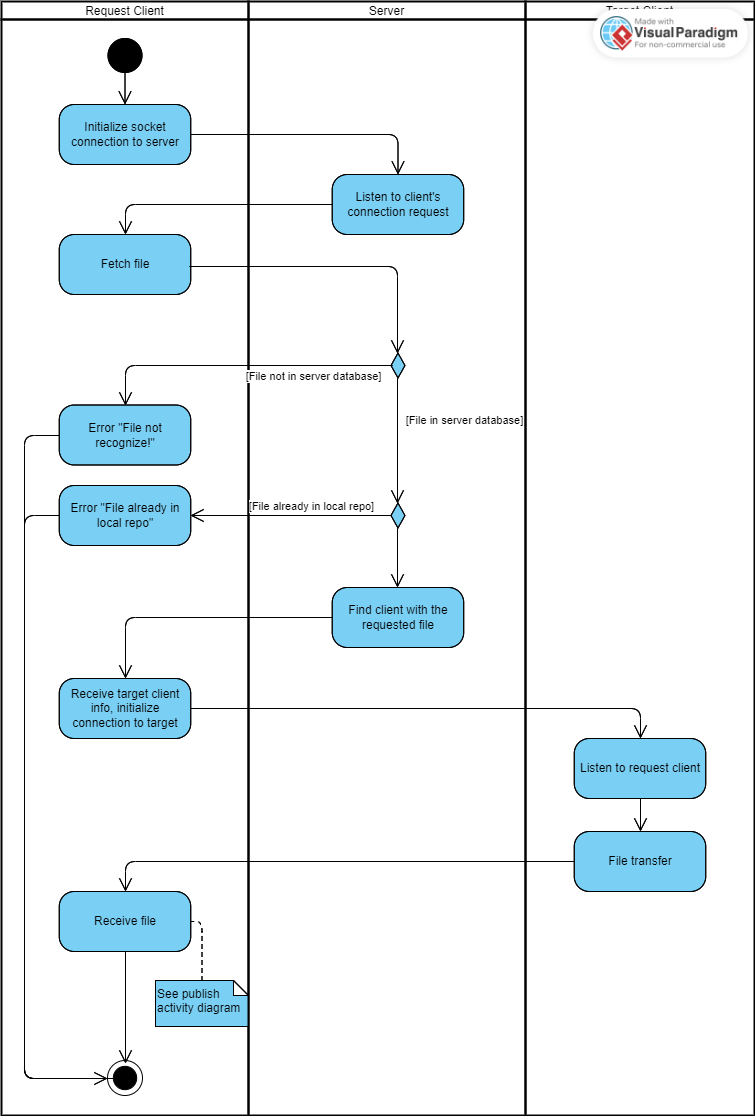
\includegraphics[width=0.7\textwidth]{images/fetch_activity_diagram.png}
			\hspace{\textwidth}
			\caption{Lược đồ hoạt động của câu lệnh \textbf{fetch \textit{fname}}}
			\label{fetch_diagram}
		\end{center}
	\end{figure}
	\subsubsection{delete \textit{fname}}
	$\indent$Thiếp lập kết nối tương tự hai câu lệnh trước. Server sẽ tiến hành kiểm tra xem file đó có trong local repo của client hay không. Trường hợp có thì tiến hành xóa khỏi dữ liệu server, trường hợp không thì đóng kết nối và kết thúc.
	\begin{figure}[h]
		\begin{center}
			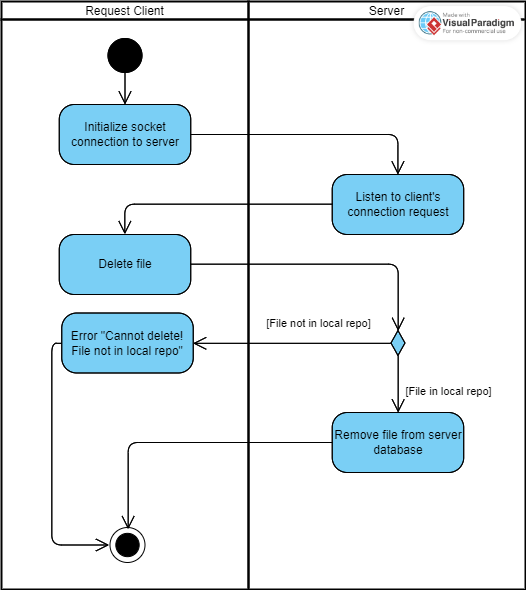
\includegraphics[width=0.7\textwidth]{images/delete_activity_diagram.png}
			\hspace{\textwidth}
			\caption{Lược đồ hoạt động của câu lệnh \textbf{delete \textit{fname}}}
			\label{delete_diagram}
		\end{center}
	\end{figure}
	\subsubsection{discover \textit{hostname}}
	$\indent$Từ dữ liệu server đã nhận được từ việc các client publish file của mình lên. Server kiểm tra xem \textit{hostname} đã từng kết nối chưa. Trường hợp có rồi và đã publish file thì cho ra danh sách các file trong local repo, còn nếu chưa publish file thì cũng thông báo ra màn hình. Trường hợp chưa từng kết nối thì báo lỗi và kết thúc. Câu lệnh này chỉ cần duy nhất server thực hiện, không cần kết nối với client nào.
	\begin{figure}[h]
		\begin{center}
			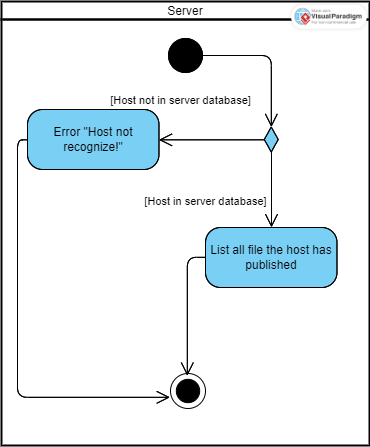
\includegraphics[width=0.7\textwidth]{images/discover_activity_diagram.png}
			\hspace{\textwidth}
			\caption{Lược đồ hoạt động của câu lệnh \textbf{discover \textit{hostname}}}
			\label{discover_diagram}
		\end{center}
	\end{figure}
	\subsubsection{ping \textit{hostname}}
	$\indent$Dùng để ping tới một \textit{hostname} đã kết nối với server từ trước. Nếu đã kết nối từ trước thì thực hiện việc trao đổi message xác nhận cho nhau. Còn nếu chưa thì báo lỗi và kết thúc.
	\begin{figure}[h]
		\begin{center}
			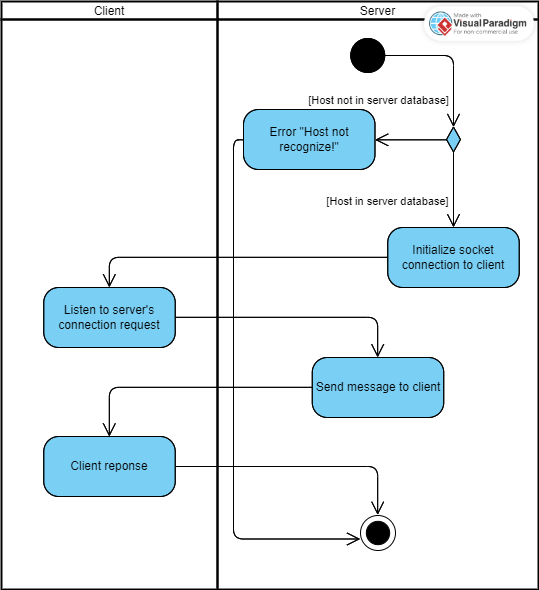
\includegraphics[width=0.7\textwidth]{images/ping_activity_diagram.png}
			\hspace{\textwidth}
			\caption{Lược đồ hoạt động của câu lệnh \textbf{ping \textit{hostname}}}
			\label{ping_diagram}
		\end{center}
	\end{figure}
	\newpage
	%%%%%%%%%%%%%%%%%%%%%%%%%%%%%%%%%
	
	
	\section{Implement and validation}
	\subsection{Manual document}
	...
	
	\subsection{Source code}
	...
	
	\subsection{Validation and evaluation}
	...
	
	\begin{thebibliography}{80}
		
		
		\bibitem{bib1}
		...
		
		
		\bibitem{bib2}
		...
		
		
	\end{thebibliography}
\end{document}

